\chapter{Theorie}
\label{kap-theorie}

Nach den einleitenden Bemerkungen in Kapitel \ref{kap-einleitung} mit der fundamentalen Gleichung 
 \eqref{gl-erwartungswert} geht es jetzt weiter. Die Definition des Kreises ist illustriert 
in Abb.~\ref{fig-kreis}.

\begin{figure}
% Rather than specifying figure widths in raw terms, like centimetres, or docu-
% ment parameters like \textwidth, it’s nice to be able to have a more semantic
% reference. Having a few standard width also helps to keep things looking con-
% sistent through the document. For these reasons, hepthesis provides four
% standard figure widths, \smallfigwidth, \mediumfigwidth, \largefigwidth
% and \hugefigwidth, which are defined in terms of the text width and chosen
% to avoid overflows. Use them like this:
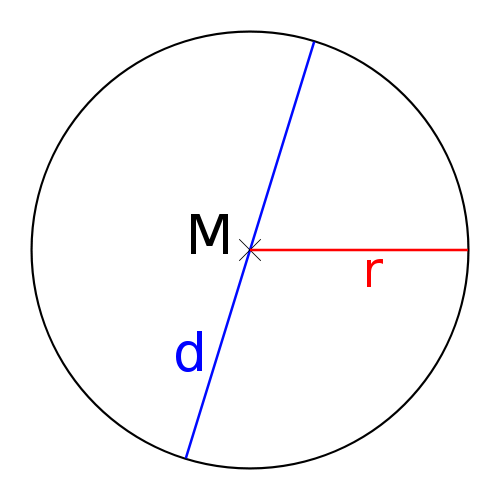
\includegraphics[width=\mediumfigwidth]{bilder/kreis.png}
\caption{Ein Kreis ist die Menge aller Punkte, die von einem gemeinsamen Mittelpunkt den gleichen Abstand haben.  Hier wird eine PNG-Grafik eingelesen.}
\label{fig-kreis}
\end{figure} 

\pagebreak
\section{Hamilton-Operator des Systems}
In  Abb.~\ref{fig-quadrat} wird das Quadrat gezeigt.

\begin{figure}[h]
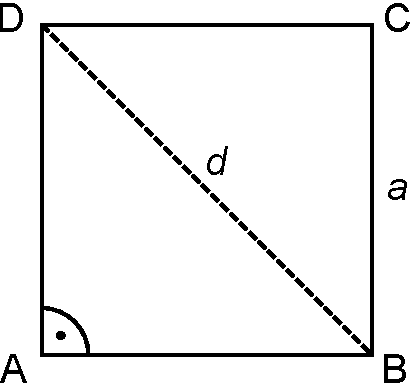
\includegraphics[width=\smallfigwidth]{bilder/quadrat.pdf}
\caption{Ein Quadrat ist etwas völlig anderes als ein Kreis (siehe Abb.\ \ref{fig-kreis}). 
Hier wird ein PDF-File als Grafik eingelesen.}
\label{fig-quadrat}
\end{figure} 



\section{Störungstheoretische Betrachtung}
